% Provenance (never printed): cycle 3 / 6e "La planete Terre" (rocks and
% minerals; the three rock families; recognising common rocks); see
% sources/book1/PROVENANCE.md. Book 1, grade 6, chapter 3.
% Vocabulary guard: "magma" not before g7.2 (here "molten rock");
% "sediment" not before g7.4 (here "grains of sand and mud").
\chapter{الصخور والمعادن}\label{ch:g6:rocks-and-minerals}

ينحني سامي فوق سطح المطبخ وفي يده عدسة مكبرة. والحجر المصقول، الذي يبدو
رماديًا من بعيد، يتحول إلى حشد من النقاط: نقاط وردية، وأخرى بيضاء، وأخرى
رمادية زجاجية، ونقاط سوداء صغيرة تلمع حين يقع عليها الضوء. ولكل نقطة
وجوه مسطحة لامعة، والنقاط متداخلة بعضها في بعض كقطع لعبة التركيب.
فما هي؟

\begin{omfigure}
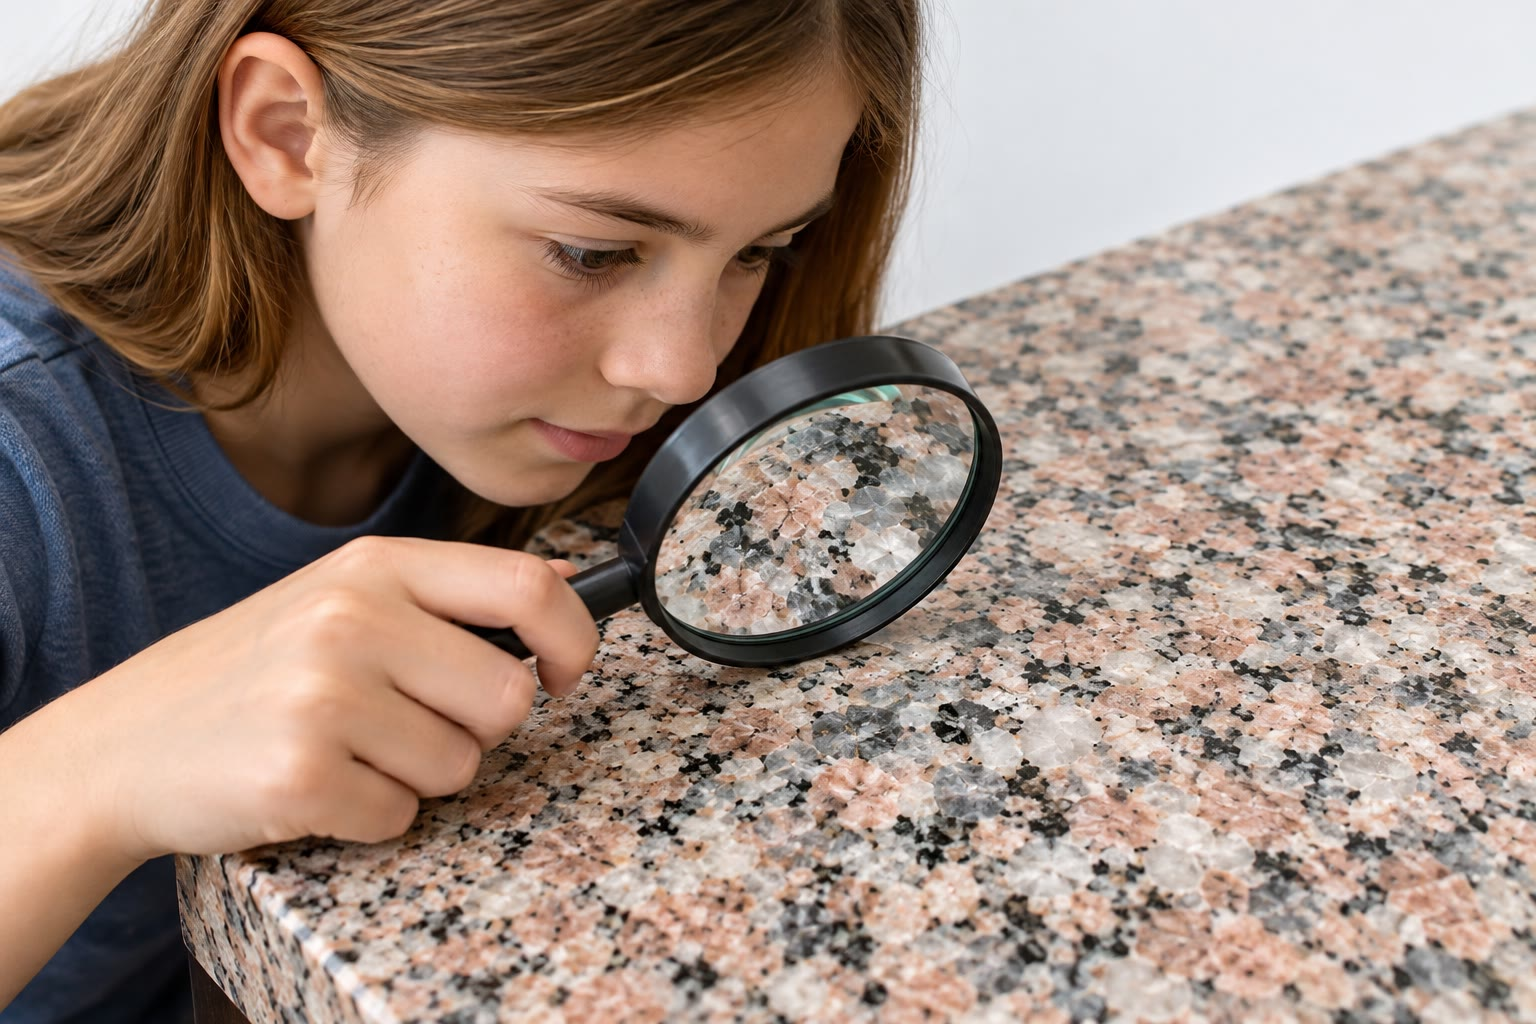
\includegraphics[width=0.6\linewidth]{images/book1/ai/g6-hand-lens-worktop.jpg}

{\small سطح حجري مرقّط في مطبخ، كما يُرى من خلال عدسة مكبرة. (رسم
بالذكاء الاصطناعي.)}
\end{omfigure}

\begin{recall}
\omterm{def:g3:stones-pebbles-sand:rock}{الصخور} هي المادة الصلبة لقشرة الأرض: يمكن أن تتكسر حجارةً، وأن تدحرجها
\omterm{def:g1:landscapes-around-us:water}{الأنهار} فتصير حصًى، وأن تُطحن فتصير \omterm{def:g3:stones-pebbles-sand:sand}{رملًا}
(\cref{ch:g3:stones-pebbles-sand}). والماء والجليد والريح تُبلي \omterm{def:g3:stones-pebbles-sand:rock}{الصخور}
(\omterm{def:g5:water-shapes-the-land:weathering}{التجوية})، وتحمل قطعها بعيدًا (\omterm{def:g5:water-shapes-the-land:erosion}{التعرية})، ثم تلقيها في مكان أبعد
(\omterm{def:g5:water-shapes-the-land:deposition}{الترسيب}) (\cref{ch:g5:water-shapes-the-land}). وعند \omterm{def:g4:volcanoes-earthquakes-first-look:volcano}{البركان}، يخرج \omterm{def:g3:stones-pebbles-sand:rock}{الصخر}
المنصهر \omterm{def:g4:volcanoes-earthquakes-first-look:eruption}{حممًا} (\cref{ch:g4:volcanoes-earthquakes-first-look}).
\end{recall}

\section{الصخر مكوَّن من معادن}

نقاط سطح المطبخ \omterm{def:g6:rocks-and-minerals:mineral}{معادن}، والحجر غرانيت.

\begin{definition}[المعدن]\label{def:g6:rocks-and-minerals:mineral}
\emph{المعدن}\index{معدن} مادة صلبة طبيعية، لا تصنعها الكائنات الحية،
تركيبها ثابت لا يتغير، وذراتها مرتبة ترتيبًا منتظمًا. و\emph{\omterm{def:g3:stones-pebbles-sand:rock}{الصخر}}
يتكون من معدن واحد، أو في أكثر الأحيان من عدة معادن ملتصقة بعضها
ببعض.
% ledger: usgs:mineral-rock
\end{definition}

يتكون الغرانيت أساسًا من ثلاثة \omterm{def:g6:rocks-and-minerals:mineral}{معادن}: \emph{الفلسبار} (وردي أو أبيض)،
و\emph{الكوارتز} (رمادي زجاجي) و\emph{الميكا} (سوداء أو فضية، في رقائق
رقيقة لامعة). وتتكون \omterm{def:g3:stones-pebbles-sand:rock}{صخور} أخرى من \omterm{def:g6:rocks-and-minerals:mineral}{معدن} واحد: فالحجر الجيري، مثلًا، يكاد
يتكون من الكالسيت وحده.
% ledger: nps:granite-minerals, usgs:mineral-rock

\begin{omfigure}
\begin{minipage}[c]{0.5\linewidth}\centering
\begin{tikzpicture}
  \begin{axis}[axis equal image, hide axis, width=\linewidth,
      xmin=0, xmax=6, ymin=0, ymax=4]
    \addplot[fill=orange!35!pink, draw=black!55, line width=0.4pt]
      table {figdata/out/grade-6-granite_mosaic-feldspar.dat};
    \addplot[fill=black!12, draw=black!55, line width=0.4pt]
      table {figdata/out/grade-6-granite_mosaic-quartz.dat};
    \addplot[fill=black!85, draw=black!55, line width=0.4pt]
      table {figdata/out/grade-6-granite_mosaic-mica.dat};
  \end{axis}
\end{tikzpicture}

{\small \tikz\fill[orange!35!pink, draw=black!55] (0,0) rectangle (0.25,0.18); فلسبار\quad
\tikz\fill[black!12, draw=black!55] (0,0) rectangle (0.25,0.18); كوارتز\quad
\tikz\fill[black!85] (0,0) rectangle (0.25,0.18); ميكا}
\end{minipage}\hfill
\begin{minipage}[c]{0.46\linewidth}\centering
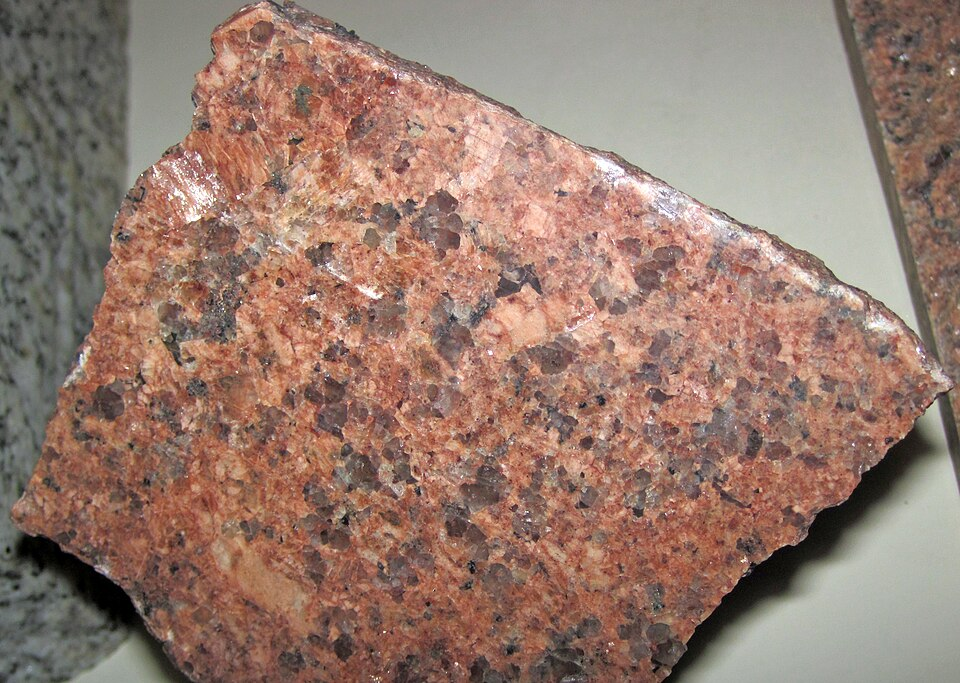
\includegraphics[width=\linewidth]{images/book1/g6-granite.jpg}
\end{minipage}

\smallskip
{\small إلى اليمين: الغرانيت مرسومًا فسيفساءً من الحبيبات، كل حبيبة منها
\omterm{def:g6:rocks-and-minerals:mineral}{معدن} واحد (صورة مكبَّرة، لا تحترم المقياس). إلى اليسار: غرانيت وردي
حقيقي، بحجم اليد تقريبًا. (صورة: جيمس سانت~جون، CC BY 2.0، عبر ويكيميديا كومنز.)}
% ledger: nps:granite-minerals, commons:jsj-rocks (figdata/grade-6/granite_mosaic.py)
\end{omfigure}

\section{البلورات}

تحت العدسة، تُظهر كثير من حبيبات \omterm{def:g6:rocks-and-minerals:mineral}{المعادن} وجوهًا مسطحة لامعة وحوافَّ
مستقيمة. وحيث يجد \omterm{def:g6:rocks-and-minerals:mineral}{المعدن} متسعًا لينمو بحرية، في تجويف داخل \omterm{def:g3:stones-pebbles-sand:rock}{الصخر}، فإنه
يكوّن بلورة: جسمًا صلبًا شكله منتظم تحده وجوه مسطحة. ويأتي شكلها من
الترتيب المنتظم لذراتها، وهو ما تدرسه كتب الكيمياء. فبلورة الكوارتز،
مثلًا، عمود له ستة أوجه ينتهي برأس مدبب؛ وبلورة الميكا تنفلق صفائح
أرق من الورق.

\begin{omfigure}
\begin{minipage}[c]{0.2\linewidth}\centering
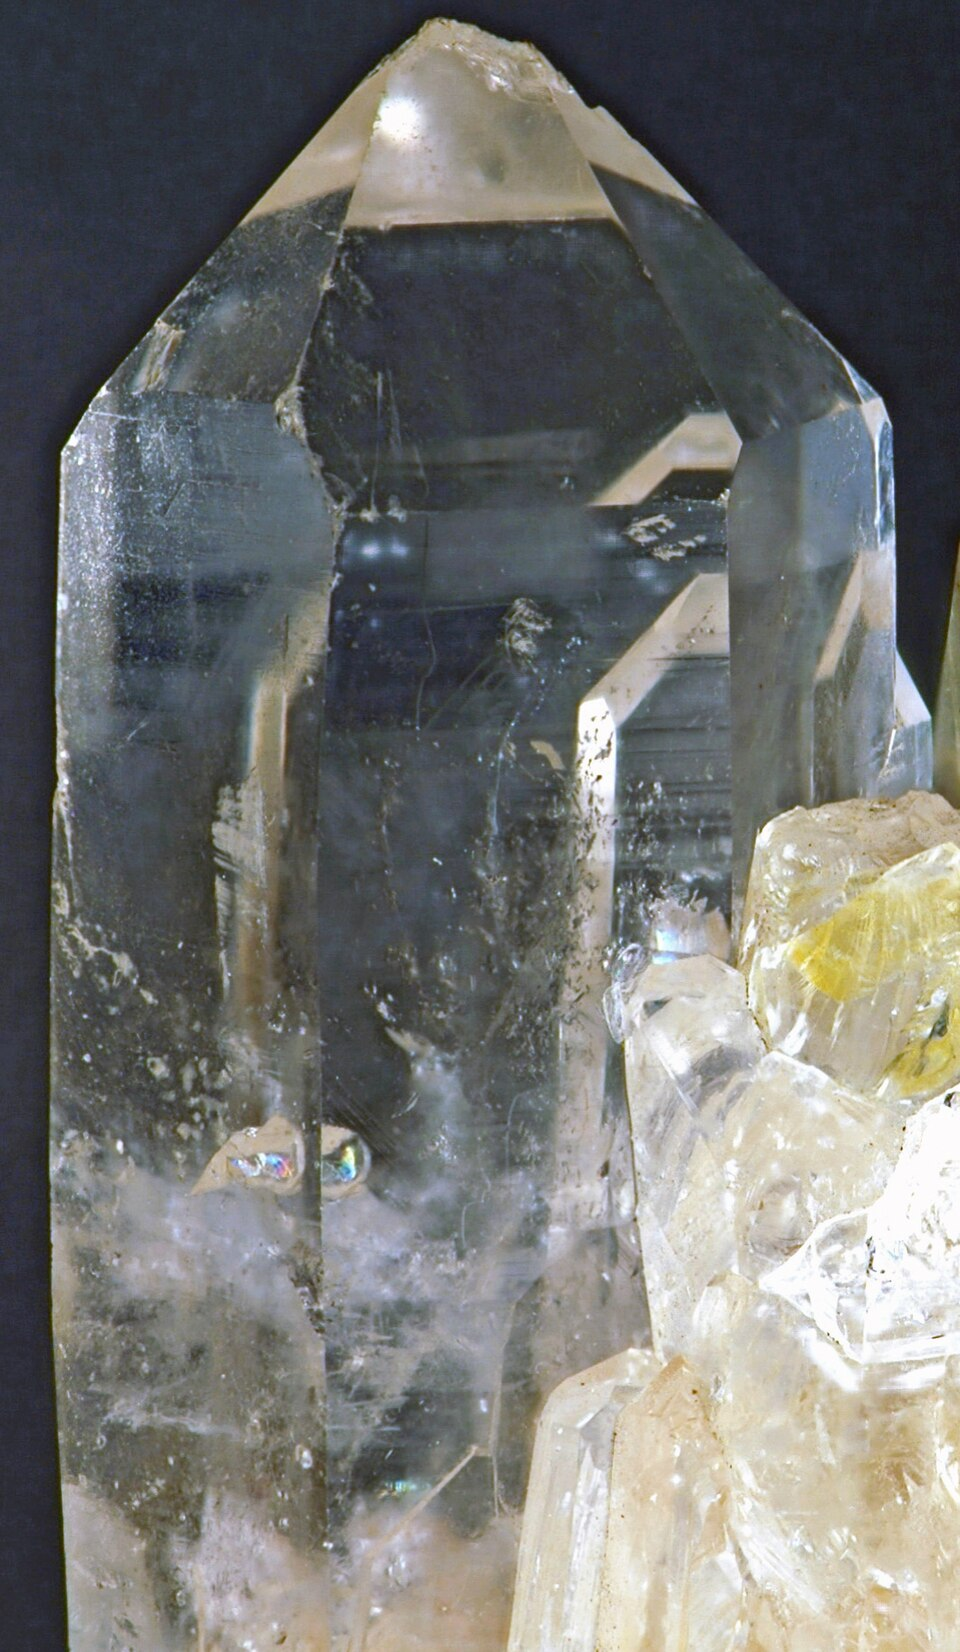
\includegraphics[height=4.2cm]{images/book1/g6-quartz.jpg}
\end{minipage}\hfill
\begin{minipage}[c]{0.44\linewidth}\centering
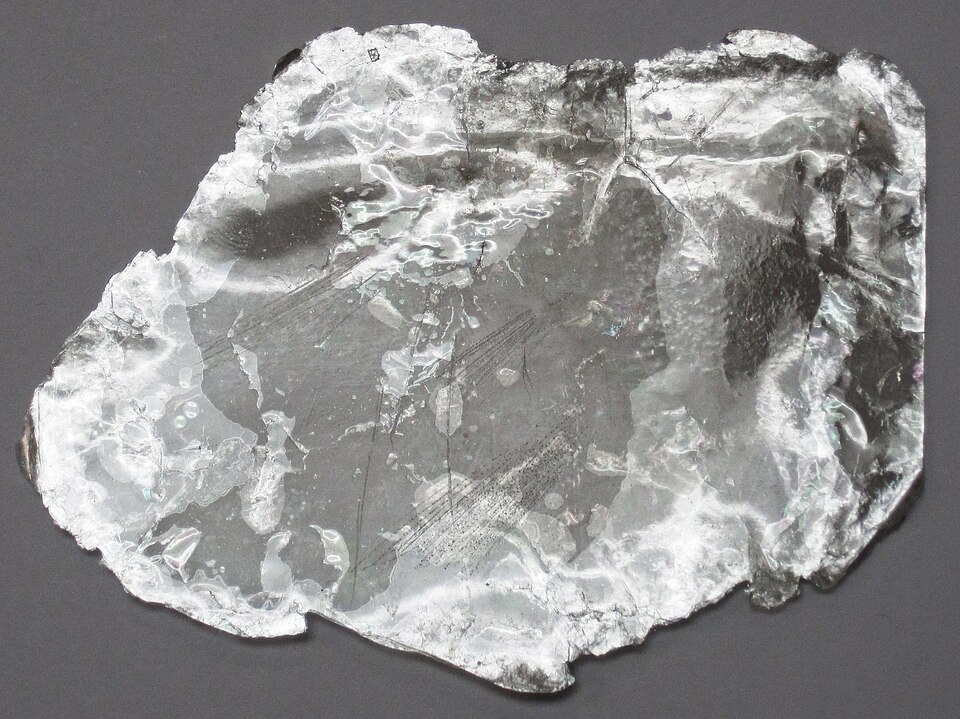
\includegraphics[height=4.2cm]{images/book1/g6-mica.jpg}
\end{minipage}\hfill
\begin{minipage}[c]{0.28\linewidth}
{\small إلى اليمين: بلورة كوارتز، بوجوهها المسطحة. إلى اليسار: صفيحة من
الميكا، وهي \omterm{def:g6:rocks-and-minerals:mineral}{معدن} ينفلق رقائق رقيقة جدًا. (صور: جيمس
سانت~جون، CC BY 2.0، عبر ويكيميديا كومنز.)}
% ledger: commons:jsj-rocks
\end{minipage}
\end{omfigure}

في الغرانيت، نمت الحبيبات وهي مضغوطة بعضها على بعض، فلم تتخذ أشكالًا
منتظمة: إنها متداخلة كقطع لعبة التركيب. وحجمها يروي حكاية. فالغرانيت
يتكون في أعماق الأرض، حيث يبرد \omterm{def:g3:stones-pebbles-sand:rock}{الصخر} المنصهر ببطء شديد: فتجد حبيباته
وقتًا لتكبر حتى تُرى بالعين. أما \omterm{def:g3:stones-pebbles-sand:rock}{الصخر} المنصهر الذي يبرد بسرعة على
السطح، \omterm{def:g4:volcanoes-earthquakes-first-look:eruption}{حممًا}، فيعطي صخورًا حبيباتها أصغر من أن تُرى.
% ledger: usgs:mineral-rock

\section{عائلات الصخور الثلاث}

يصنّف الجيولوجيون \omterm{def:g3:stones-pebbles-sand:rock}{الصخور} في ثلاث عائلات، لا بحسب لونها، بل بحسب الطريقة
التي تكونت بها.

\begin{definition}[عائلات الصخور الثلاث]\label{def:g6:rocks-and-minerals:rock-families}
\emph{الصخر الناري}\index{صخر ناري} يتكون حين يبرد \omterm{def:g3:stones-pebbles-sand:rock}{الصخر} المنصهر
ويتصلب: الغرانيت في أعماق الأرض، والبازلت من \omterm{def:g4:volcanoes-earthquakes-first-look:eruption}{الحمم}.
و\emph{الصخر الرسوبي}\index{صخر رسوبي} يتكون على سطح الأرض من حبيبات
\omterm{def:g3:stones-pebbles-sand:sand}{الرمل} \omterm{def:g3:stones-pebbles-sand:sand}{والوحل}، أو من أصداف الكائنات الحية، التي تترسب في طبقات ثم
تتصلب: الحجر الرملي، والسجّيل، والحجر الجيري.
و\emph{الصخر المتحول}\index{صخر متحول} \omterm{def:g3:stones-pebbles-sand:rock}{صخر} تحوّل، دون أن ينصهر، بفعل
الحرارة والضغط في أعماق الأرض: الرخام (من الحجر الجيري)، والأردواز (من
السجّيل).
% ledger: usgs:mineral-rock, usgs:sedimentary, usgs:metamorphic, geo:marble, geo:slate
\end{definition}

وتسمية \emph{النارية} مأخوذة من النار، وكذلك اسمها في اللغات الأوروبية،
المشتق من الكلمة اللاتينية الدالة على النار. وكثيرًا ما تُظهر \omterm{def:g6:rocks-and-minerals:rock-families}{الصخور الرسوبية} طبقات، بعضها
فوق بعض، كصفحات كتاب. \omterm{def:g6:rocks-and-minerals:rock-families}{والصخور المتحولة} كثيرًا ما تكون مضغوطة مطوية؛
وبعضها، مثل الأردواز، ينفلق صفائح مسطحة.
% ledger: usgs:mineral-rock, usgs:sedimentary, usgs:metamorphic

كثير من \omterm{def:g6:rocks-and-minerals:rock-families}{الصخور الرسوبية} مكوَّن من الحبيبات التي فرزتها بحسب حجمها في
\cref{ch:g3:stones-pebbles-sand}: \omterm{def:g3:stones-pebbles-sand:pebble}{الحصى} \omterm{def:g3:stones-pebbles-sand:pebble}{والحصباء}، \omterm{def:g3:stones-pebbles-sand:sand}{والرمل}، \omterm{def:g3:stones-pebbles-sand:sand}{والوحل}. وحين
تُدفن الحبيبات، تفقد ماءها ويلصقها بعضها ببعض ملاط طبيعي. وحجم الحبيبات
هو الذي يعطي \omterm{def:g3:stones-pebbles-sand:rock}{الصخر} اسمه.
% ledger: usgs:sedimentary, usgs:wentworth

\begin{omfigure}
\begin{tikzpicture}[
    col/.style={draw=black!60, rounded corners=2pt, minimum width=3.6cm, minimum height=1.9cm},
    lab/.style={font=\scriptsize, align=center}]
  % gravel -> conglomerate
  \node[col, fill=omLithCongl!50] (g) at (0,0) {};
  \foreach \x/\y/\r in {-1.2/0.4/0.32, -0.4/-0.3/0.4, 0.5/0.35/0.3, 1.25/-0.35/0.33, 0.2/-0.55/0.18, -1.3/-0.5/0.22}
    \fill[gray!55, draw=black!60] (\x,\y) circle (\r);
  \node[lab, above=2pt] at (g.north) {\textbf{حصباء}\\ \foreignlanguage{arabic}{أكثر من 2~مليمتر}};
  \node[lab, below=3pt] (cg) at (g.south) {\foreignlanguage{arabic}{$\downarrow$ دفن والتحام}\\ \textbf{رصيص}};
    % sand -> sandstone
  \pgfmathsetseed{7}

  \node[col, fill=omLithSand!60] (s) at (4.2,0) {};
  \foreach \i in {1,...,70} \fill[brown!60!black] ({4.2+1.65*rand},{0.82*rand}) circle (0.045);
  \node[lab, above=2pt] at (s.north) {\textbf{رمل}\\ \foreignlanguage{arabic}{من 2~مليمتر إلى $\frac{1}{16}$~مليمتر}};
  \node[lab, below=3pt] at (s.south) {\foreignlanguage{arabic}{$\downarrow$ دفن والتحام}\\ \textbf{حجر رملي}};
  % mud -> shale
  \node[col, fill=omLithShale!70] (m) at (8.4,0) {};
  \foreach \y in {-0.75,-0.5,...,0.8} \draw[black!35, line width=0.3pt] (6.75,\y) -- (10.05,\y);
  \node[lab, above=2pt] at (m.north) {\textbf{وحل}، أي غرين وطين\\ \foreignlanguage{arabic}{أقل من $\frac{1}{16}$~مليمتر}};
  \node[lab, below=3pt] at (m.south) {\foreignlanguage{arabic}{$\downarrow$ دفن وانضغاط}\\ \textbf{سجّيل}};
\end{tikzpicture}

{\small ثلاثة \omterm{def:g6:rocks-and-minerals:rock-families}{صخور رسوبية} سُميت بحسب حجم حبيباتها (الحبيبات مكبَّرة
كثيرًا؛ \omterm{def:g3:stones-pebbles-sand:sand}{الرمل} مرسوم بمقياس الصندوق، \omterm{def:g3:stones-pebbles-sand:pebble}{والحصباء} أكبر).}
% ledger: usgs:wentworth, usgs:sedimentary
\end{omfigure}

\begin{inthefield}[قراءة حجارة المدينة]
المدن مجموعات \omterm{def:g3:stones-pebbles-sand:rock}{صخور} في الهواء الطلق. امشِ مع شخص بالغ بمحاذاة الأسوار
القديمة، والدرج، والتماثيل، وواجهات الكنائس، والأرصفة، وانظر عن قرب، دون
أن تخدش شيئًا أو تكسره. بعض حواف الأرصفة والدرجات من الغرانيت: ابحث فيه عن الكوارتز الزجاجي والميكا اللامعة. وكثير من الأسوار والواجهات القديمة من الحجر الجيري أو الحجر الرملي: ابحث عن الأصداف، أو امسح بطرف إصبعك فتاتة ساقطة من
الحجر الرملي لتحس \omterm{def:g3:stones-pebbles-sand:sand}{بالرمل}. وقد تكون السقوف من الأردواز، منفلقة صفائح رقيقة.
دوّن في دفتر مكان كل حجر، ولونه، وحبيباته، والعائلة التي تظن أنه
ينتمي إليها؛ والصورة الفوتوغرافية تساعد على المقارنة لاحقًا بجدول هذا
الفصل.
\end{inthefield}

\section{دورة الصخور}

\omterm{def:g3:stones-pebbles-sand:rock}{الصخور} ليست خالدة. \omterm{def:g1:landscapes-around-us:landform}{فجبل} الغرانيت تتلفه \omterm{def:g5:water-shapes-the-land:weathering}{التجوية} ببطء؛ وتحمل \omterm{def:g1:landscapes-around-us:water}{الأنهار}
حبيباته إلى \omterm{def:g2:water-on-earth:ocean}{البحر} فتترسب هناك في طبقات؛ وكلما دُفنت الطبقات أعمق فأعمق
تصلبت حتى صارت حجرًا رمليًا. وإذا حُمل الحجر الرملي إلى أعماق أبعد، حوّلته
الحرارة والضغط إلى \omterm{def:g6:rocks-and-minerals:rock-families}{صخر متحول}؛ وفي أعماق أبعد أيضًا، قد ينصهر، فيصنع
\omterm{def:g3:stones-pebbles-sand:rock}{الصخر} المنصهر حين يبرد \omterm{def:g3:stones-pebbles-sand:rock}{صخرًا} ناريًا جديدًا. وشيئًا فشيئًا، على مدى ملايين
السنين، تظل مادة \omterm{def:g3:stones-pebbles-sand:rock}{الصخور} تدور وتدور.
% ledger: usgs:sedimentary, usgs:metamorphic

\begin{definition}[دورة الصخور]\label{def:g6:rocks-and-minerals:rock-cycle}
\emph{دورة الصخور}\index{دورة الصخور} هي الرحلة التي لا تنتهي، والتي
تتحول بها \omterm{def:g3:stones-pebbles-sand:rock}{صخور} كل عائلة ببطء إلى \omterm{def:g3:stones-pebbles-sand:rock}{صخور} العائلتين الأخريين: \omterm{def:g5:water-shapes-the-land:weathering}{بالتجوية}
\omterm{def:g5:water-shapes-the-land:erosion}{والتعرية} على السطح، وبالدفن والتصلب، وبالحرارة والضغط، وبالانصهار
والتبرد.
\end{definition}

\begin{omfigure}
\begin{tikzpicture}[
    fam/.style={draw, rounded corners=4pt, thick, align=center, minimum width=3.2cm,
                minimum height=1.0cm, font=\small\bfseries},
    stage/.style={draw, dashed, rounded corners=4pt, align=center, minimum width=3.0cm,
                  minimum height=0.9cm, font=\small},
    arr/.style={-{Stealth[length=2.6mm]}, thick},
    lab/.style={font=\scriptsize, align=center, fill=white, inner sep=1.5pt}]
  \node[fam, fill=omLithGranite!60] (ign) at (0,3.6) {صخور نارية\\[-1pt]{\normalfont\scriptsize غرانيت، بازلت}};
  \node[stage, fill=orange!15] (grains) at (6.6,3.6) {حبيبات رمل\\ووحل};
  \node[fam, fill=omLithSand!70] (sed) at (6.6,0) {صخور رسوبية\\[-1pt]{\normalfont\scriptsize حجر رملي، سجّيل، حجر جيري}};
  \node[fam, fill=omLithSchist!60] (met) at (0,0) {صخور متحولة\\[-1pt]{\normalfont\scriptsize رخام، أردواز}};
  \node[stage, fill=red!12] (melt) at (-4.2,1.8) {صخر منصهر\\في الأعماق};
  \draw[arr] (ign) -- node[lab, above] {تجوية\\وتعرية} (grains);
  \draw[arr] (grains) -- node[lab, right] {ترسّب في طبقات\\ثم دفن وتصلّب} (sed);
  \draw[arr] (sed) -- node[lab, below=2pt] {حرارة وضغط\\في الأعماق} (met);
  \draw[arr] (met) -- node[lab, below left] {انصهار} (melt);
  \draw[arr] (melt) -- node[lab, above left] {تبرّد} (ign);
  \draw[arr, black!55] (met.north east) to[bend left=12] node[lab, pos=0.45, left=4pt, text=black!60] {تجوية} ([xshift=-6pt]grains.south west);
  \draw[arr, black!55] (sed.north west) to[bend left=10] (grains.south west);
\end{tikzpicture}

{\small \omterm{def:g6:rocks-and-minerals:rock-cycle}{دورة الصخور}. تستغرق كل خطوة من آلاف السنين إلى ملايينها. وكل \omterm{def:g3:stones-pebbles-sand:rock}{صخر}
يصعد إلى السطح يمكن أن تتلفه \omterm{def:g5:water-shapes-the-land:weathering}{التجوية} (الأسهم
الرمادية).}
% ledger: usgs:sedimentary, usgs:metamorphic, usgs:mineral-rock
\end{omfigure}

\section{التعرف على الصخور الشائعة}

إليك سبعة \omterm{def:g3:stones-pebbles-sand:rock}{صخور} كثيرًا ما نصادفها في المباني والأرصفة
والمناظر الطبيعية.

\begin{omfigure}
\newcommand{\gsixrock}[2]{\begin{minipage}[t]{0.235\linewidth}\centering
  \includegraphics[width=\linewidth, height=0.72\linewidth, keepaspectratio=false]{images/book1/#1}\\[1pt]
  {\footnotesize #2}\end{minipage}}
\gsixrock{g6-granite.jpg}{غرانيت}\hfill
\gsixrock{g6-basalt.jpg}{بازلت}\hfill
\gsixrock{g6-sandstone.jpg}{حجر رملي}\hfill
\gsixrock{g6-limestone.jpg}{حجر جيري (فيه أصداف)}\par\medskip
\gsixrock{g6-shale.jpg}{سجّيل}\hspace{0.02\linewidth}%
\gsixrock{g6-marble.jpg}{رخام}\hspace{0.02\linewidth}%
\gsixrock{g6-slate-roof.jpg}{أردواز، على سقف}

\medskip
{\small سبعة \omterm{def:g3:stones-pebbles-sand:rock}{صخور} شائعة. (صور: جيمس سانت~جون، CC BY 2.0؛ السقف:
أويفيند هولمستاد، CC0؛ عبر ويكيميديا كومنز.)}
% ledger: commons:jsj-rocks, commons:roof-slates
\end{omfigure}

\begin{center}
\small
\begin{tabular}{>{\raggedright\arraybackslash}p{0.13\linewidth}>{\raggedright\arraybackslash}p{0.15\linewidth}>{\raggedright\arraybackslash}p{0.6\linewidth}}
\hline
\omterm{def:g3:stones-pebbles-sand:rock}{الصخر} & العائلة & ما نبحث عنه\\
\hline
غرانيت & ناري & حبيبات كبيرة متعددة الألوان: فلسبار وردي أو أبيض، وكوارتز رمادي زجاجي، وميكا سوداء لامعة\\
بازلت & ناري & رمادي داكن إلى أسود، حبيباته أصغر من أن تُرى، وفيه غالبًا ثقوب صغيرة مستديرة خلّفتها فقاعات الغاز\\
حجر رملي & رسوبي & حبيبات \omterm{def:g3:stones-pebbles-sand:sand}{رمل} نحسّها باللمس، خشن كورق الصنفرة\\
حجر جيري & رسوبي & فاتح اللون، فيه غالبًا أصداف؛ يُحدث فورانًا تحت قطرة من حمض مخفف\\
سجّيل & رسوبي & ناعم جدًا وطري، مكوَّن من \omterm{def:g3:stones-pebbles-sand:sand}{وحل} متصلب (طين)؛ في طبقات رقيقة\\
رخام & متحول & أبيض أو ملوّن، مكوَّن من بلورات لامعة تتلألأ كالسكر؛ يُحدث فورانًا تحت الحمض\\
أردواز & متحول & رمادي، ناعم جدًا، ينفلق صفائح رقيقة صلبة مسطحة\\
\hline
\end{tabular}
% ledger: nps:granite-minerals, geo:basalt, usgs:sedimentary, geo:limestone, geo:marble, geo:slate
\end{center}

\begin{safety}
لا يُجري اختبارَ الحمض إلا شخص بالغ، بنظارات واقية وقفازين، وبحمض مخفف
جدًا. لا تتذوق أبدًا \omterm{def:g3:stones-pebbles-sand:rock}{صخرًا} أو مسحوقًا، ولا تكسر \omterm{def:g3:stones-pebbles-sand:rock}{الصخور} أبدًا بأداة: فالنظر
من خلال عدسة مكبرة يخبرنا بالكثير.
% ledger: geo:limestone
\end{safety}

المفتاح قائمة من الأسئلة، لكل منها جوابان، تقود خطوة بعد خطوة إلى
اسم \omterm{def:g3:stones-pebbles-sand:rock}{الصخر}.

\begin{omfigure}
\begin{tikzpicture}[
    q/.style={draw, rounded corners=3pt, fill=omRecall!10, align=center, text width=3.7cm,
              font=\scriptsize, inner sep=3pt},
    r/.style={draw, rounded corners=3pt, thick, fill=omLithSand!40, font=\scriptsize\bfseries,
              align=center, minimum width=1.7cm, inner sep=3pt},
    arr/.style={-{Stealth[length=2mm]}, thick}, yn/.style={font=\scriptsize\itshape, fill=white, inner sep=1pt}]
  \node[q] (q1) at (0,0) {\foreignlanguage{arabic}{هل يُحدث فورانًا تحت قطرة من حمض مخفف؟}};
  \node[q] (q2) at (-3.4,-1.6) {\foreignlanguage{arabic}{هل ترى أصدافًا، أو هل يبدو باهتًا ناعمًا؟}};
  \node[r] (lime) at (-4.8,-3.4) {حجر جيري};
  \node[r, align=center] (marb) at (-2.0,-3.4) {رخام\\[-1pt]{\normalfont\tiny بلورات لامعة}};
  \node[q] (q3) at (3.2,-1.6) {\foreignlanguage{arabic}{هل ترى حبيبات متعددة الألوان، وردية ورمادية وسوداء؟}};
  \node[r] (gran) at (6.9,-1.6) {غرانيت};
  \node[q] (q4) at (3.2,-3.2) {\foreignlanguage{arabic}{داكن، حبيباته أصغر من أن تُرى، وفيه ثقوب صغيرة مستديرة؟}};
  \node[r] (bas) at (6.9,-3.2) {بازلت};
  \node[q] (q5) at (3.2,-4.8) {\foreignlanguage{arabic}{خشن كورق الصنفرة، مكوَّن من حبيبات رمل؟}};
  \node[r] (sand) at (6.9,-4.8) {حجر رملي};
  \node[q] (q6) at (3.2,-6.4) {\foreignlanguage{arabic}{صلب، ينفلق صفائح رقيقة مسطحة؟}};
  \node[r] (slat) at (6.9,-6.4) {أردواز};
  \node[r] (shal) at (3.2,-7.8) {سجّيل};
  \draw[arr] (q1) -| node[yn, pos=0.25] {نعم} (q2);
  \draw[arr] (q1) -| node[yn, pos=0.25] {لا} (q3);
  \draw[arr] (q2.south-|lime) -- node[yn, right] {نعم} (lime);
  \draw[arr] (q2.south-|marb) -- node[yn, right] {لا} (marb);
  \foreach \a/\b in {q3/gran, q4/bas, q5/sand, q6/slat}{\draw[arr] (\a) -- node[yn, above] {نعم} (\b);}
  \foreach \a/\b in {q3/q4, q4/q5, q5/q6, q6/shal}{\draw[arr] (\a) -- node[yn, right] {لا} (\b);}
\end{tikzpicture}

{\small مفتاح لتعرّف \omterm{def:g3:stones-pebbles-sand:rock}{صخور} الجدول السبعة. ابدأ من الأعلى وأجب عن كل سؤال
بنعم أو لا.}
% ledger: geo:limestone, geo:marble, nps:granite-minerals, geo:basalt, usgs:sedimentary, geo:slate
\end{omfigure}

\paragraph{الصلادة.} وهناك دليل آخر يساعد على التعرف على \omterm{def:g6:rocks-and-minerals:mineral}{المعدن}: مدى
سهولة خدشه.

\begin{definition}[الصلادة وسلم موس]\label{def:g6:rocks-and-minerals:hardness}
\emph{صلادة}\index{صلادة} \omterm{def:g6:rocks-and-minerals:mineral}{المعدن} هي مدى مقاومته للخدش: \omterm{def:g6:rocks-and-minerals:mineral}{فالمعدن} يخدش كل
\omterm{def:g6:rocks-and-minerals:mineral}{معدن} أطرى منه، ويخدشه كل \omterm{def:g6:rocks-and-minerals:mineral}{معدن} أصلد منه. و\emph{سلم موس}\index{سلم موس}
يرتّب الصلادة من 1 إلى 10 بعشرة \omterm{def:g6:rocks-and-minerals:mineral}{معادن} مرجعية، من التلك (1)، وهو
أطراها، إلى الماس (10)، وهو أصلدها.
% ledger: nps:mohs-ladder, nps:mohs-testers
\end{definition}

\begin{omfigure}
\begin{tikzpicture}[x=1cm, y=0.62cm]
  \draw[thick, black!60] (0,0.5) -- (0,10.5);
  \foreach \n/\m in {1/تلك, 2/جبس, 3/كالسيت, 4/فلوريت, 5/أباتيت,
                     6/فلسبار الأورثوكلاز, 7/كوارتز, 8/توباز, 9/كوراندوم, 10/ماس}{
    \fill[omRecall!25, draw=black!50] (-0.32,\n-0.32) rectangle (0.32,\n+0.32);
    \node[font=\scriptsize\bfseries] at (0,\n) {\n};
    \node[font=\scriptsize, anchor=east] at (-0.5,\n) {\m};}
  \foreach \v/\t in {2.5/ظفر, 3.5/قطعة نقود نحاسية, 5.5/زجاج, 6.5/مسمار فولاذي}{
    \draw[red!70!black, thick] (0.4,\v) -- (1.0,\v);
    \node[font=\scriptsize, red!70!black, anchor=west] at (1.05,\v) {\foreignlanguage{arabic}{\t: نحو \babelsublr{\v}}};}
  \node[font=\scriptsize\itshape, anchor=south] at (0,10.6) {أصلد};
  \node[font=\scriptsize\itshape, anchor=north] at (0,0.4) {أطرى};
  \node[font=\scriptsize, align=left, anchor=west, text width=6.2cm] at (4.3,5.5)
    {\foreignlanguage{arabic}{الظفر يخدش التلك والجبس، لكنه لا يخدش الكالسيت. وقطعة النقود
     النحاسية تخدش الكالسيت. والكوارتز يخدش الزجاج والفولاذ؛ ولا يخدش الكوارتزَ أيٌّ من الأدوات الأربع. والميكا، وصلادتها من 2 إلى 3، يكاد
     الظفر يخدشها.}};
\end{tikzpicture}

{\small \omterm{def:g6:rocks-and-minerals:hardness}{سلم موس} (على اليسار: \omterm{def:g6:rocks-and-minerals:mineral}{المعادن} المرجعية العشرة) وأربع أدوات اختبار
من الحياة اليومية (على اليمين، بالأحمر).}
% ledger: nps:mohs-ladder, nps:mohs-testers, geo:mica-hardness
\end{omfigure}

\begin{method}[اختبار الخدش]\label{met:g6:rocks-and-minerals:scratch}
\begin{enumerate}
  \item حاول أن تخدش \omterm{def:g6:rocks-and-minerals:mineral}{المعدن} بظفرك، ثم بقطعة نقود نحاسية. (أما الزجاج
        والفولاذ فلا يستعملهما إلا شخص بالغ.)
  \item امسح الأثر بإصبعك: الخدش الحقيقي يبقى، أما أثر المسحوق المتخلف
        عن أداة الاختبار فيزول.
  \item تقع \omterm{def:g6:rocks-and-minerals:hardness}{الصلادة} بين \omterm{def:g6:rocks-and-minerals:hardness}{صلادة} أصلد أداة لا تخدشه \omterm{def:g6:rocks-and-minerals:hardness}{وصلادة} أطرى أداة
        تخدشه.
\end{enumerate}
\end{method}

\begin{example}[كوارتز أم كالسيت؟]\label{ex:g6:rocks-and-minerals:quartz-calcite}
معدنان أبيضان متشابهان. الأول تخدشه قطعة نقود نحاسية: \omterm{def:g6:rocks-and-minerals:hardness}{صلادته} أقل من
3.5؛ إنه الكالسيت (3). والثاني لا يخدشه مسمار فولاذي ويخدش الزجاج:
\omterm{def:g6:rocks-and-minerals:hardness}{صلادته} أكثر من 6.5؛ ومن بين \omterm{def:g6:rocks-and-minerals:mineral}{المعادن} المرجعية، إنه
الكوارتز (7).
% ledger: nps:mohs-ladder, nps:mohs-testers
\end{example}

\section{تمارين}

\begin{exercise}[$\star$]\label{exo:g6:rocks-and-minerals:1}
إلى أي عائلة ينتمي كل \omterm{def:g3:stones-pebbles-sand:rock}{صخر} من هذه \omterm{def:g3:stones-pebbles-sand:rock}{الصخور}: الغرانيت، والحجر الرملي، والرخام،
والبازلت، والحجر الجيري، والأردواز؟
\end{exercise}

\begin{exercise}[$\star$]\label{exo:g6:rocks-and-minerals:2}
هل الكوارتز \omterm{def:g6:rocks-and-minerals:mineral}{معدن} أم \omterm{def:g3:stones-pebbles-sand:rock}{صخر}؟ والغرانيت؟ اشرح الفرق في
جملة واحدة.
\end{exercise}

\begin{exercise}[$\star$]\label{exo:g6:rocks-and-minerals:3}
رتّب هذه \omterm{def:g6:rocks-and-minerals:mineral}{المعادن} من الأطرى إلى الأصلد: الكوارتز، والتلك، والماس،
والكالسيت. أيها يستطيع أن يخدشها كلها؟
\end{exercise}

\begin{exercise}[$\star$]\label{exo:g6:rocks-and-minerals:4}
انقل وأكمل بالكلمات \emph{التبرد}، \emph{الحرارة والضغط}،
\emph{\omterm{def:g5:water-shapes-the-land:weathering}{التجوية}}: «يصير \omterm{def:g3:stones-pebbles-sand:rock}{الصخر} المنصهر \omterm{def:g3:stones-pebbles-sand:rock}{صخرًا} ناريًا عن طريق \ldots{} ويصير
الحجر الجيري رخامًا عن طريق \ldots{} ويتحول الغرانيت إلى حبيبات \omterm{def:g3:stones-pebbles-sand:sand}{رمل}
عن طريق \ldots»
\end{exercise}

\begin{exercise}[$\star\star$]\label{exo:g6:rocks-and-minerals:5}
استعمل المفتاح. (أ) \omterm{def:g3:stones-pebbles-sand:rock}{صخر} لا يُحدث فورانًا تحت الحمض؛ وهو داكن، حبيباته
أصغر من أن تُرى، وفيه ثقوب صغيرة مستديرة. (ب) \omterm{def:g3:stones-pebbles-sand:rock}{صخر} يُحدث فورانًا تحت الحمض
ومكوَّن من بلورات لامعة تتلألأ كالسكر. (ج) \omterm{def:g3:stones-pebbles-sand:rock}{صخر} لا يُحدث فورانًا؛ وهو خشن
كورق الصنفرة. سمِّ كل \omterm{def:g3:stones-pebbles-sand:rock}{صخر}.
\end{exercise}

\begin{exercise}[$\star\star$]\label{exo:g6:rocks-and-minerals:6}
\omterm{def:g6:rocks-and-minerals:mineral}{معدن} تخدشه قطعة نقود نحاسية ولا يخدشه الظفر. بين أي قيمتين من قيم
\omterm{def:g6:rocks-and-minerals:hardness}{الصلادة} يقع؟ وأي \omterm{def:g6:rocks-and-minerals:mineral}{معدن} مرجعي من \omterm{def:g6:rocks-and-minerals:mineral}{معادن} \omterm{def:g6:rocks-and-minerals:hardness}{سلم موس}
يمكن أن يكون؟
\end{exercise}

\begin{exercise}[$\star\star$]\label{exo:g6:rocks-and-minerals:7}
% exercise data: figdata/grade-6/granite_mosaic.py (33 / 21 / 6 grains)
في رسم الغرانيت في هذا الفصل 60 حبيبة: 33 من الفلسبار، و21 من
الكوارتز، و6 من الميكا. ما النسبة المئوية لحبيبات الكوارتز؟ والفلسبار؟
والميكا؟ تحقق من أن مجموع النسب المئوية الثلاث يساوي
100~\%.
\end{exercise}

\begin{exercise}[$\star\star$]\label{exo:g6:rocks-and-minerals:8}
الغرانيت والبازلت كلاهما \omterm{def:g6:rocks-and-minerals:rock-families}{صخر ناري}. لماذا نستطيع أن نرى حبيبات الغرانيت
بأعيننا، ولا نستطيع أن نرى حبيبات البازلت؟
\end{exercise}

\begin{exercise}[$\star\star$]\label{exo:g6:rocks-and-minerals:9}
يتكوّن الرخام من الحجر الجيري. (أ) إلى أي عائلة ينتمي كل منهما؟
(ب) ماذا حدث للحجر الجيري حتى تحول إلى رخام؟ (ج) لماذا يُحدث كلاهما
فورانًا تحت الحمض؟
\end{exercise}

\begin{exercise}[$\star\star$]\label{exo:g6:rocks-and-minerals:10}
باستعمال \omterm{def:g6:rocks-and-minerals:hardness}{سلم موس}: (أ) هل يستطيع الكوارتز أن يخدش قنينة زجاجية؟ (ب) وهل
يستطيع الفلوريت ذلك؟ (ج) هل يستطيع مسمار فولاذي أن يخدش الفلسبار؟
\end{exercise}

\begin{exercise}[$\star\star\star$]\label{exo:g6:rocks-and-minerals:11}
احكِ رحلة حبيبة كوارتز، في خمس خطوات، من \omterm{def:g1:landscapes-around-us:landform}{جبل} غرانيتي إلى \omterm{def:g6:rocks-and-minerals:rock-families}{صخر متحول}.
سمِّ العملية في كل خطوة، وعائلة \omterm{def:g3:stones-pebbles-sand:rock}{الصخر} في البداية
وفي النهاية.
\end{exercise}

\begin{exercise}[$\star\star\star$]\label{exo:g6:rocks-and-minerals:12}
\omterm{def:g6:rocks-and-minerals:mineral}{معدن} رمادي زجاجي لا يخدشه مسمار فولاذي، ويخدش الزجاج، ويخدشه
التوباز. (أ) ما \omterm{def:g6:rocks-and-minerals:hardness}{صلادته} على \omterm{def:g6:rocks-and-minerals:hardness}{سلم موس}؟ سمِّه. (ب) تتدحرج حبيبات \omterm{def:g3:stones-pebbles-sand:sand}{الرمل}
سنوات طويلة بفعل الأمواج \omterm{def:g1:landscapes-around-us:water}{والأنهار}. اشرح، مستعينًا \omterm{def:g6:rocks-and-minerals:hardness}{بصلادة} هذا \omterm{def:g6:rocks-and-minerals:mineral}{المعدن}،
لماذا تبقى حبيباته مدة أطول بكثير من حبيبات الكالسيت أو
الميكا.
\end{exercise}

\section{مسألة: حجارة ساحة البلدة}

\begin{problem}[{مسألة نهاية الأسبوع --- صخور ساحة البلدة، وأصلد معدن
فيها، وكم عائلة من عائلات الصخور موجودة فيها}]
\label{pb:g6:rocks-and-minerals:1}
% ledger: nps:granite-minerals, geo:limestone, geo:slate, geo:marble, nps:mohs-ladder, nps:mohs-testers, geo:mica-hardness
في رحلة مدرسية، يتأمل التلاميذ حجارة ساحة البلدة القديمة (تأمُّلًا فقط:
لا أحد يكسر النُّصُب أو يخدشها). وقد أحضر المعلم قطعًا مفككة من الحجارة
نفسها من ورشة النحّات، من أجل اختبارات
\omterm{def:g6:rocks-and-minerals:hardness}{الصلادة}.

\smallskip
\noindent\textbf{النافورة}: في حوضها حبيبات كبيرة، وردية وبيضاء،
        ورمادية زجاجية، وسوداء لامعة.
\textbf{البلاط}: ألواح فاتحة اللون نرى فيها أصدافًا متحجرة صغيرة؛
        وقطرة من حمض مخفف، يضعها المعلم على قطعة مفككة،
        تُحدث فورانًا.
\textbf{سقف دار البلدية}: صفائح رقيقة مسطحة رمادية من حجر
        ناعم الحبيبات جدًا.
\textbf{التمثال}: حجر أبيض مكوَّن من بلورات لامعة
        تتلألأ كالسكر؛ ويُحدث فورانًا هو أيضًا.

\medskip
\noindent\textbf{الجزء الأول --- النافورة والبلاط والسقف.}
\begin{enumerate}
  \item سمِّ \omterm{def:g3:stones-pebbles-sand:rock}{صخر} النافورة وعائلته. وسمِّ معادنه
        الثلاثة.
  \item سمِّ \omterm{def:g3:stones-pebbles-sand:rock}{صخر} البلاط وعائلته. ماذا كانت الأصداف قبل أن تصير
        في الحجر؟
  \item سمِّ \omterm{def:g3:stones-pebbles-sand:rock}{صخر} السقف وعائلته. ومن أي \omterm{def:g3:stones-pebbles-sand:rock}{صخر}
        تكوّن؟
  \item سمِّ \omterm{def:g3:stones-pebbles-sand:rock}{صخر} التمثال وعائلته. ومن أي \omterm{def:g3:stones-pebbles-sand:rock}{صخر}
        تكوّن؟
\end{enumerate}

\medskip
\noindent\textbf{الجزء الثاني --- اختبار الصلادة.}
\begin{enumerate}[resume]
  \item يحاول المعلم أن يخدش حبيبة رمادية زجاجية من النافورة
        بمسمار فولاذي: لا خدش. والحبيبة تخدش الزجاج. ما
        هذا \omterm{def:g6:rocks-and-minerals:mineral}{المعدن}، وما \omterm{def:g6:rocks-and-minerals:hardness}{صلادته}؟
  \item الحبيبات الوردية يخدشها المسمار الفولاذي ولا يخدشها الزجاج.
        بين أي قيمتين تقع \omterm{def:g6:rocks-and-minerals:hardness}{صلادتها}؟ وأي \omterm{def:g6:rocks-and-minerals:mineral}{معدن} من \omterm{def:g6:rocks-and-minerals:mineral}{معادن}
        \omterm{def:g6:rocks-and-minerals:hardness}{سلم موس} هو؟
  \item الرقائق السوداء يكاد الظفر يخدشها. أي
        \omterm{def:g6:rocks-and-minerals:mineral}{معدن} هي؟
  \item هل تستطيع قطعة نقود نحاسية أن تخدش البلاط؟ اشرح مستعينًا \omterm{def:g6:rocks-and-minerals:hardness}{بصلادة}
        الكالسيت.
\end{enumerate}

\medskip
\noindent\textbf{الجزء الثالث --- دورة الصخور.}
\begin{enumerate}[resume]
  \item بعد قرون من \omterm{def:g4:clouds-rain-snow:precipitation}{المطر}، فقد التمثال تفاصيله الدقيقة.
        أي عملية من عمليات \omterm{def:g6:rocks-and-minerals:rock-cycle}{دورة الصخور} تعمل هنا؟
  \item جاء غرانيت النافورة من \omterm{def:g1:landscapes-around-us:landform}{جبل}. على مدى ملايين
        السنين، ماذا يمكن أن يحدث لحبيبات الكوارتز في ذلك \omterm{def:g1:landscapes-around-us:landform}{الجبل}،
        وفي أي \omterm{def:g3:stones-pebbles-sand:rock}{صخر} يمكن أن ينتهي بها المطاف؟
  \item كم عائلة من عائلات \omterm{def:g3:stones-pebbles-sand:rock}{الصخور} الثلاث موجودة في الساحة؟
        سمِّ \omterm{def:g3:stones-pebbles-sand:rock}{صخر} كل عائلة أو صخورها.
  \item ما \omterm{def:g6:rocks-and-minerals:hardness}{صلادة} موس لأصلد \omterm{def:g6:rocks-and-minerals:mineral}{معدن} نجده في
        حجارة الساحة؟
\end{enumerate}
\end{problem}
